\documentclass[11pt]{article}
\usepackage[margin=0.92in]{geometry}
\usepackage{amsmath,amssymb,amsthm,booktabs,graphicx}
\usepackage[hidelinks]{hyperref}
\newtheorem{theorem}{Theorem}
\newtheorem{lemma}{Lemma}
\newcommand{\E}{\mathcal{E}}
\newcommand{\R}{\mathcal{R}}
\newcommand{\dd}{\Delta}
\title{Certifying changes in group rate gaps\\from a shared statistical release}
\author{Yunjie Guo \and Hanqing Yang\thanks{Corresponding author: \texttt{hanqing.yang189@gmail.com}. Both authors: Independent Researcher, Suzhou, China.}}
\date{}
\begin{document}
\maketitle
\begin{abstract}
How much could reweighting schools change a group proficiency gap when only intervals for the school counts are public? We derive attainable endpoints over a shared latent table and an unknown replacement mix, with a quadratic-time algorithm that returns an extremizing mix. We compare threshold decisions against linear-time bounds adapted from fractional programming and total-variation inequalities. For a 10\% replacement and a five-percentage-point tolerance, a vertex scan with a curvature allowance settled 387 of 417 California districts. Three simpler shared-table bounds together settled all 417. In a geographic replication they settled 505 of 506 Texas districts; a rational Bernstein bound settled the remaining case. Across both states, 412 districts stayed within tolerance and 511 admitted a violating mix. The contribution is a sharp finite-table reference and an empirical account of when standard bounds suffice. The direction and size of the gaps pertain to standardized compositions with fixed school outcomes.
\end{abstract}

\section{The audit question}
A school district knows how many English learners and other students took a mathematics assessment at each school. The public release gives bands for proficiency. Could a shift of one tenth of tested volume among schools move the district proficiency gap by more than five percentage points, with school conditions fixed? The same unobserved proficient counts enter the baseline and the alternative. Allowing different counts in those two calculations gives an apparent range of changes even when the school mix stays fixed.

We assume that the two group denominators at each site are known and its outcome counts are constrained by the release. We pursue three quantities: the largest attainable increase, the largest attainable decrease, and the error incurred by checking just one recipient site at a time. They refer to the observed finite table with standardized weights. A small certified change can coexist with a large baseline gap.

Rate decomposition has a long history. Kitagawa separates composition and rate effects for specified populations \cite{kitagawa}. Giguere et al.\ provide learning guarantees under demographic shift \cite{giguere}; Cherian and Cand\`es develop simultaneous statistical audits \cite{cherian}. These address generalization or sampling uncertainty. Our uncertainty set consists of the same unknown finite cells used under two weight vectors, one itself unknown. Kallus, Mao and Zhou bound disparities with missing protected class information \cite{kallus}; here group sizes are observed. Zaccour, Binns and Rocher study audit accuracy from privacy-perturbed aggregates \cite{zaccour}. We instead bound a change over all admissible recipient mixes from a single release. Dobra and Fienberg derive sharp feasible cell bounds from published margins \cite{dobra}. Given such bounds, our target is a change in an aggregate contrast over a common table and possibly unknown site weights. Repeated inputs can inflate interval calculations \cite{interval}. Anchored replacement has the usual $\epsilon$-contamination form \cite{berger}. Single linear fractions, the fixed-table two-ratio edge reduction, and sharp total-variation bounds for reweighting all have established theory \cite{charnes,cambini,cohen}. Our specialization eliminates latent rate corners along each edge, returns an attaining table and mix, and bounds the loss from restricting witnesses to single sites. We compare it with direct applications of these existing bounds and with a rational Bernstein enclosure. The empirical question is which decisions require sharp endpoints once the strongest shared-table screens have run.

\section{Finite-table estimand}
Let $s=1,\dots,K$ index sites and $g=1,0$ two groups. Site proportions $q_{gs}>0$ are known, with $q_{1s}+q_{0s}=1$. Let $r_{gs}\in[l_{gs},h_{gs}]$ denote outcome rates. We begin with a rectangular release permitting every combination of feasible cells, including their endpoints. Section~5 adds within-site sum constraints. The results also apply to integer counts in these intervals divided by their known denominators. Write $b$ for the reference site weights on the simplex and define
\[
 B_g=\sum_s b_s q_{gs},\qquad
 M_g(w;r)=\frac{\sum_s w_s q_{gs}r_{gs}}{\sum_s w_s q_{gs}},\qquad
 G(w;r)=M_1(w;r)-M_0(w;r).
\]
A replacement fraction $\rho\in[0,1]$ gives $w=(1-\rho)b+\rho u$, where $u$ can be any distribution over the sites. All site laws remain fixed. This family is nested in $\rho$ and includes $b$ at every radius. It describes replacement proportional to the anchor on the removed side; arbitrary targeted removal would give a different uncertainty set. The quantity of interest is
\[
 \E_\rho=\{G((1-\rho)b+\rho u;r)-G(b;r): u\in\dd_{K-1},\ r\in\R\}.
\]
For each table, continuity in $u$ gives an interval containing zero. The union therefore fills the interval between the two attainable extrema even for discrete count sets.

\section{Exact endpoints in quadratic time}
\begin{lemma}
For fixed rates, each extreme signed change admits a replacement distribution supported on at most two sites.
\end{lemma}
\begin{proof}
Fix the target group-1 mass at its optimizing value. The other group mass is its complement. Both denominators are then constant, so maximizing the change is linear in $u$ over the simplex subject to at most one additional affine equality. An extreme solution has at most two nonzero entries. The same argument applies after negating the contrast. Compactness and positivity ensure existence.
\end{proof}
This is the two-ratio edge property specialized to complementary denominators. The remaining difficulty is the number of possible tables: an eight-site panel alone can have $2^{16}$ distinct rate corners.

\begin{theorem}
Over the common rectangular release, each endpoint of $\E_\rho$ can be found in $O(K^2)$ real arithmetic operations and $O(K)$ working memory. The algorithm returns the recipient pair and mixing fraction, from which an attaining table can be reconstructed.
\end{theorem}
\begin{proof}
It suffices to maximize in each orientation. Absorb the sign of each group into its rates, reversing interval endpoints as necessary. Now both signed terms are added. Lemma 1 applies at an optimizing table, so examine $u_i=t,\ u_j=1-t$. For each group let $U_g(t)=tq_{gi}+(1-t)q_{gj}$ and $D_g=(1-\rho)B_g+\rho U_g$. The coefficient of a signed rate in the change is
\[
 c_{gs}=\frac{\rho q_{gs}}{B_g D_g}\{B_g u_s-b_s U_g(t)\}.
\]
Use the high endpoint when the coefficient is positive and the low endpoint otherwise. Every site outside the pair can use its low signed rate, including at ties. The four expressions in braces on the pair are affine in $t$. Their interior roots split the unit interval into at most five pieces. Corners on adjacent pieces give the same value at a switch.

On each piece let $\beta_g$ be the anchor mean under its chosen signed rates. The objective is the sum over the groups of
\[
 F_g(t)=\frac{\rho\{t q_{gi}(r_{gi}-\beta_g)+(1-t)q_{gj}(r_{gj}-\beta_g)\}}{D_g(t)}.
\]
Precompute the all-low anchor totals and update just two sites to obtain $\beta_g$ in constant time. Each derivative is $C_g/D_g(t)^2$ for a constant $C_g$. When the constants have opposite signs, the derivative vanishes where
$\sqrt{|C_1|}\,D_0(t)=\sqrt{|C_0|}\,D_1(t)$, a linear equation. An identically zero derivative or a constant piece requires only the endpoints. Otherwise evaluate the interior root if present and both boundaries. Compare all pairs in both orientations. A single site or zero replacement has zero change. All rate choices used by the calculation are attainable.
\end{proof}

\section{A linear-time enclosure and its accuracy}
An analyst can screen a large network by testing each single recipient site plus the unchanged mix. Let $[L_v,H_v]$ be their joint inner range, including the full release uncertainty. With $q_{g-}=\min_s q_{gs}$, $q_{g+}=\max_s q_{gs}$, and $D_{g\pm}=(1-\rho)B_g+\rho q_{g\pm}$, set
\[
 A=\sum_g
 \frac{\sqrt{D_{g+}}-\sqrt{D_{g-}}}{\sqrt{D_{g+}}+\sqrt{D_{g-}}}
 \frac{\rho q_{g+}}{D_{g+}}\,
 \big(\max_s h_{gs}-\min_s l_{gs}\big).
\]
\begin{theorem}
$[L_v,H_v]\subseteq\E_\rho\subseteq[L_v-A,H_v+A]$. Both intervals cost $O(K)$ to compute. For fixed positive anchor group masses $A=O(\rho^2)$ as $\rho\downarrow0$. The worst-case order of the single-recipient error cannot be improved.
\end{theorem}
\begin{proof}
Fix a rate table and any pair. Along the edge, the target mean in group $g$ is a mixture of the endpoint means $m_i,m_j$ with weight $\alpha=tD_i/(tD_i+(1-t)D_j)$ on $m_i$. Its deviation from the linear chord is $(\alpha-t)(m_i-m_j)$. Maximizing $|\alpha-t|$ by differentiation gives $|\sqrt{D_i}-\sqrt{D_j}|/(\sqrt{D_i}+\sqrt{D_j})$, bounded by the first factor in $A$. This square-root factor also follows from the sharp total-variation bound for reweighting two-point laws \cite{cohen}. The single-recipient mean $m_i$ moves from the fixed baseline toward $r_{gi}$ by fraction $\lambda_i=\rho q_{gi}/D_i\le\rho q_{g+}/D_{g+}$. All such means lie between the baseline moved by the maximum fraction toward the smallest and the largest feasible rates. Their span is at most the product of the last two factors. Summing bounds the chord error for either signed contrast. Baseline subtraction leaves the error unchanged. Apply Theorem 1 to the optimizing table and pair. Single-site extrema use a common default corner and at most one correction per group. The square-root factor equals $\rho(q_{g+}-q_{g-})/(\sqrt{D_{g+}}+\sqrt{D_{g-}})^2$, yielding the asserted order.

For necessity, anchor on site 3, take $q_1=(.9,.1,.5)$ and let both groups have rates $(1,0,.5)$. The best single-site increase is $.8\rho(1-\rho)/(1-.64\rho^2)$. Equal replacement from sites 1 and 2 attains $.8\rho$, exceeding the single-site value by $.8\rho^2+O(\rho^3)$. All group shares are positive.
\end{proof}

\paragraph{Other comparators.}
Separate-table subtraction takes the maximum target gap minus the minimum baseline gap for the upper endpoint, and reverses the choices for the lower endpoint. It is an honest outer bound under rectangular releases. At zero shift its width equals twice the baseline gap range. A second bound evaluates both sharp endpoints for midpoint rates and pads each by $\sum_g\lambda_{g+}\max_s(h_{gs}-l_{gs})$. Indeed the total variation between baseline and target \emph{conditional} site weights is at most $\lambda_{g+}$, and the midpoint errors have range at most the maximum cell width. This comparator already cancels at zero replacement. Theorem 2 instead controls the curvature of the objective even when the rates are known exactly.


For the empirical comparison we also bound each group fraction separately, transfer both fractions to a common measure using total variation, or bound the ratio of the two denominators. Each calculation uses one pass over sites. Their endpoint intersection remains linear time. A quadratic-time rational Bernstein enclosure supplies a stronger polynomial comparison. Appendix~\ref{sec:competitors} derives each bound over the same released cells and shows that TV transfer already gives a second-order allowance.

\section{When do the marginal ranges suffice?}
A public total can constrain two site counts $(x_s,y_s)$ to an integer rectangle intersected with a sum band. Projecting the polygon onto each axis keeps each count's feasible range but allows some impossible pairs. We distinguish the resulting shared-table rectangle audit from separate-table subtraction, which additionally permits the baseline and target counts to differ.

For a fixed target mix $w$, let $D_g=\sum_s w_sq_{gs}$ and let $n_s$ be the combined site denominator. In the change of the group-1 minus group-0 gap the coefficients of $x_s$ and $y_s$ are, respectively,
\[
 c_s=(w_s/D_1-b_s/B_1)/n_s,\qquad
 d_s=(b_s/B_0-w_s/D_0)/n_s .
\]
For the upper endpoint the marginal rectangle selects a corner according to the signs of $c_s,d_s$. The polygon gives the same endpoint precisely when, at every site, at least one maximizing rectangle point is feasible. To see necessity, each site loss is nonnegative and adds to the total. Sufficiency follows by assembling the maximizing points; the count vertices are integral. Negate both coefficients for the lower endpoint. Opposite-sign corners are always feasible for a projected sum-band polygon (Appendix~\ref{app:totals}). When both coefficients are nonzero with the same sign, clipping the selected high--high or low--low corner strictly changes the endpoint. For $b_s>0$ these equal signs require $w_s/b_s$ to lie strictly between $D_1/B_1$ and $D_0/B_0$. This ties the potential failure to differences in how the two groups reweight the same site.

Over a family of mixes, equality at a projected extremum requires at least one optimizing mix with such a feasible maximizing table. A single incompatible witness cannot rule out another optimizer. A projected outer interval entirely inside the tolerance already certifies the decision. A feasible violating witness rules it out. For two-sided tolerance $\tau$, let $R_J,R_P$ be the larger endpoint magnitude under joint and projected constraints. The decisions differ exactly for $\tau\in[R_J,R_P)$ when $R_J<R_P$. A tighter one-sided endpoint can leave $R_J$ unchanged.

\section{External validation on published proficiency bands}
\paragraph{Release and population.}
US EDFacts publishes school-level numbers of valid mathematics assessments and proficiency percentages in bands of varying precision, with suppression for very small cells \cite{edfacts}. We used California in 2018--19, the last pre-pandemic school year. At each school the ALL and LEP all-grade rows give the total and English-learner denominators and proficiency labels. The remaining tested students form the comparison group. The ALL band restricts $x+y$, the LEP band restricts $x$, and the remaining denominator bounds $y$. These are the publisher's labels. Sharpness is conditional on these two rows and the stated decoding; the audit does not link other grade, subgroup or district tables.

We inverted a whole-percent label or range on the integer lattice, admitting both nearest-percent half ties. An explicit suppression with a known denominator admits every count. A sensitivity analysis also admits truncation before encoding. Of 1,956 reporting district identifiers, 280 lacked complete, usable two-group records at every school with an ALL row. Another 1,259 fell outside the prespecified range of 3--25 schools. The resulting 417 districts contain 3,571 schools. These are descriptive audits of released aggregates. The denominators count tests with valid scores and the contrasts freeze school-level rates. The choice of five points is illustrative.

\paragraph{Unknown recipient schools.}
We specified 10\% replacement and a five-point tolerance before inspecting district effects. Joint and projected exact search certified the same 192 districts; their primary radii agreed to numerical precision. They also agreed for all three specified tolerances at 25\% and full replacement (Table~\ref{tab:edfacts}). Full replacement could still move one endpoint inward by up to 0.156 pp without changing the maximum magnitude. Under the more permissive encoding, the two exact methods each certified 185 districts. The encoding of the public release changed more primary decisions than the choice of polygon or rectangle.

\begin{table}[ht]
\centering
\caption{Districts certified out of 417 using the nearest-percent decoding. Each entry is the count shared by projected and joint exact search; district decisions coincide individually. The last column gives the number whose two-sided radius contracts by at least 0.1 pp under joint search.}
\label{tab:edfacts}
\begin{tabular}{lrrrr}
\toprule
Comparison & 2.5 pp & 5 pp & 7.5 pp & Contraction $\ge 0.1$ pp\\
\midrule
10\% replacement &65&192&283&0\\
25\% replacement &0&38&98&0\\
Full replacement &0&0&0&0\\
Equal school weights &45&123&201&9\\
\bottomrule
\end{tabular}
\end{table}

\paragraph{How many decisions depend on the screen?}
Separate-table subtraction certified no California district and had median width 27.80 pp. Exact shared-table search certified 192, with median width 8.36 pp. This comparison shows the cost of discarding common cells. To isolate the role of the screening algorithm, we subsequently gave every method the same release, two orientations, threshold and attainable single-school witnesses (Table~\ref{tab:screens}). The chord screen's 387 first-pass decisions comprise 162 certifications out of 192 possible and all 225 violations. The groupwise bound settled 345, with 47 decisions unique to the chord screen and five unique to the groupwise comparison. The TV transfer settled 408 and the reciprocal bound 416. Relative to their intersection with the groupwise bound, the chord screen supplied zero additional decisions and left 30 more open. The median outer width of that intersection was 8.43 pp, versus 9.53 pp for the chord screen. No method issued a wrong first-pass classification against the joint exact reference.

\begin{table}[ht]
\centering
\caption{Paired first-pass decisions at 10\% replacement and a five-point tolerance. Pass means that every feasible change is within tolerance. Violation means that at least one feasible change exceeds it. The Texas comparison was fixed after the California results and before examining Texas records.}\label{tab:screens}
\begin{tabular}{lrrrrrr}
\toprule
&\multicolumn{3}{c}{California ($n=417$)}&\multicolumn{3}{c}{Texas ($n=506$)}\\
\cmidrule(lr){2-4}\cmidrule(lr){5-7}
Method & Pass & Violation & Open & Pass & Violation & Open\\
\midrule
Chord (Theorem 2)&162&225&30&197&286&23\\
Groupwise fractions&120&225&72&153&286&67\\
TV transfer&183&225&9&213&286&7\\
Reciprocal bound&191&225&1&219&286&1\\
Three linear bounds intersected&192&225&0&219&286&1\\
Degree-two Bernstein&192&225&0&220&286&0\\
\bottomrule
\end{tabular}
\end{table}

\paragraph{Geographic replication.}
We froze the same data selection and five-point decision for Texas, using the same federal archive and year. Of 1,203 reporting districts, 315 lacked complete usable records and 382 fell outside the size range. The 506 eligible districts contained 2,668 schools. The exact methods agreed on 220 certifications. The three intersected bounds left only Malakoff ISD open: their upper limit was 5.024 pp and the sharp upper endpoint was 4.911 pp. The degree-two Bernstein bound settled this decision. Across both states the three linear bounds resolved 922 of 923 primary decisions; every one of the 511 violations admitted a single-school witness. In both states the chord screen added zero decisions to the three linear bounds.

\paragraph{Cost and sensitivity.}
On the 417 prepared California inputs, median times over five warm Windows runs, including fallback, were 53 ms for the chord screen, 18 ms for the reciprocal bound, 19 ms for the three-bound intersection and 31 ms for Bernstein. Direct exact projected search took 492 ms for all districts. The chord screen alone took 8 ms. The 30 fallbacks outweighed its cheaper first pass. These times describe one implementation on districts with at most 25 schools. For the more permissive decoding, the intersection left one five-point decision open. At 25\% replacement it left four open at five points and five at 7.5 points. The replication files retain both signed endpoints and all district-level decisions.

\paragraph{A case requiring two recipients for the sharp endpoint.}
Fullerton Joint Union High (eight schools) was the only district-setting combination left open by the unsubdivided Bernstein check across the California grid. At 25\% replacement, its single-school lower extreme was $-5.446$ pp and the sharp lower endpoint was $-6.755$ pp, attained by allocating 69.15\% and 30.85\% of the incoming volume to two schools. The sharp upper endpoint was $+6.525$ pp. Both the linear intersection and the initial Bernstein interval crossed the $-7.5$ pp boundary. In an exploratory check, halving every recipient edge once and recomputing Bernstein coefficients over the shared table raised the lower bound from $-9.021$ to $-7.484$ pp, enough to certify the decision. Eight equal pieces gave $-6.802$ pp. This case distinguishes the practical need for an attaining mix from the computational demands of a binary decision.

\paragraph{A fixed standardization that exposes dependence.}
We separately compared the original student-weighted mix to equal weights per school. This is a fixed standardization and need not be a ten-percent shift. The joint radius contracted by more than $10^{-8}$ pp in 138 districts and by at least 0.1 pp in nine. The largest contraction, in West Sonoma County Union High, was from 45.821 to 45.602 pp. Only tolerances in the narrow interval between the underlying values switch that district's two-sided decision; all three specified tolerances give the same verdict.

An exploratory check asked whether the interval excludes zero. One district changed classification. In Old Adobe Union (five schools), projection gave $[-0.00775,\,2.07477]$ pp. Joint optimization gave $[0.00190,\,2.06513]$ pp, identifying a positive change. Direct rational arithmetic confirmed all four endpoints. Under the wider encoding its joint lower bound fell to $-0.05087$ pp, and no district gained a directional conclusion. This example establishes a dependence on the public count constraints with a sign margin of only 0.00190 pp.

\paragraph{Independent checks and a known-count benchmark.}
For each reported extremizing school mix, a separate calculation swept feasible integer learner counts and optimized the complementary count at its allowable endpoints. Both external result files reproduced byte-for-byte on Windows. In a separate, controlled IPEDS analysis with known source counts we tested 60 eight-institution panels. With admissions rounded to tens and institution totals published, the exact audit certified 14 of 20 small panels and the linear enclosure certified 12. Projection and joint search made all 60 decisions identically. Appendix~\ref{app:admissions} gives the rounding, release-noise and temporal checks. They use emulated disclosure rules; EDFacts supplies the native published bands.

\section{Scope and implications}
For a binary audit decision, intersecting three linear enclosures settled all but one primary case across the two states. Direct sharp search still answers a different practical question: how far can the gap move, and which mix and feasible table attain that limit? The common-cell edge calculation gives a finite answer without enumerating possible tables or choosing a subdivision accuracy. Its empirical advantage for threshold decisions is narrower than comparison with separate-table subtraction suggests. The matching $O(\rho^2)$ example quantifies the intrinsic limitation of single-site witnesses; the TV comparator attains the same asymptotic order. Neither the rate nor the observed first-pass percentage establishes an advantage of the chord allowance. Both states share one disclosure system and year, with complete-coverage and size restrictions. The proportion resolved can vary with the tolerance, replacement share and reporting rules.

Sharpness is relative to the stated disclosure rules. The polygon extension accommodates an exact within-site total. Cross-site outcome totals, unavailable focal group denominators, or common noisy margins change the feasible set further. Additional constraints may tighten the bounds or require another algorithm. The two-group formulation covers a prespecified pair after conditioning on its combined population; a multi-group audit needs a clear definition of the deployment weights. The finite-table analysis assigns no sampling confidence to future rates. Future use needs a defensible replacement radius, a justified fixed-site model and clarity about repeated persons across sites.

\paragraph{Availability and declarations.}
The repository contains the frozen design, pinned public inputs, code, witnesses, result tables and verification output. The admissions follow-ups and the external validation followed the original admissions study. We fixed the external population, two composition questions, tolerances, and size criterion before inspecting district effects. The direction check and the California screen comparisons are exploratory. The Texas protocol and all its methods were frozen after the California comparison and before inspecting Texas records. The subsequent Bernstein subdivision check uses the unresolved California cases. \href{https://github.com/fightforbelief/p7-shared-release-audit}{Replication repository}. The authors received no specific funding and declare no competing interests.

\begin{thebibliography}{10}
\raggedright
\bibitem{kitagawa} E. M. Kitagawa. Components of a difference between two rates. \emph{Journal of the American Statistical Association}, 50:1168--1194, 1955. \href{https://doi.org/10.1080/01621459.1955.10501299}{doi:10.1080/01621459.1955.10501299}.
\bibitem{giguere} S. Giguere, B. Metevier, Y. Brun, B. C. da Silva, P. S. Thomas, and S. Niekum. Fairness guarantees under demographic shift. \emph{ICLR}, 2022. \href{https://people.cs.umass.edu/~brun/pubs/Giguere22iclr.pdf}{Author manuscript}.
\bibitem{cherian} J. J. Cherian and E. J. Cand\`es. Statistical inference for fairness auditing. \emph{JMLR}, 25(149):1--49, 2024. \href{https://www.jmlr.org/papers/v25/23-0739.html}{Journal article}.
\bibitem{kallus} N. Kallus, X. Mao, and A. Zhou. Assessing algorithmic fairness with unobserved protected class using data combination. \emph{Management Science}, 68(3):1959--1981, 2022. \href{https://doi.org/10.1287/mnsc.2020.3850}{doi:10.1287/mnsc.2020.3850}.
\bibitem{zaccour} J. Zaccour, R. Binns, and L. Rocher. Access denied: Meaningful data access for quantitative algorithm audits. \emph{CHI}, 2025. \href{https://doi.org/10.1145/3706598.3713963}{Publisher record}.
\bibitem{dobra} A. Dobra and S. E. Fienberg. Bounds for cell entries in contingency tables given marginal totals and decomposable graphs. \emph{PNAS}, 97(22):11885--11892, 2000. \href{https://doi.org/10.1073/pnas.97.22.11885}{Publisher record}.
\bibitem{interval} A. Gray, M. de Angelis, E. Patelli, and S. Ferson. Bivariate dependency tracking in interval arithmetic. \emph{Mechanical Systems and Signal Processing}, 186:109771, 2023. \href{https://doi.org/10.1016/j.ymssp.2022.109771}{Publisher record}.
\bibitem{cohen} S. N. Cohen and E. Fausti. Hyperbolic contractivity and the Hilbert metric on probability measures. \href{https://arxiv.org/abs/2309.02413}{arXiv:2309.02413}, 2023, revised 2024.
\bibitem{cambini} A. Cambini, L. Martein, and S. Schaible. On maximizing a sum of ratios. \emph{Journal of Information and Optimization Sciences}, 10(1):65--79, 1989. \href{https://arpi.unipi.it/handle/11568/14015}{Author record}.
\bibitem{berger} J. O. Berger and L. M. Berliner. Robust Bayes and empirical Bayes analysis with $\epsilon$-contaminated priors. \emph{Annals of Statistics}, 14:461--486, 1986. \href{https://www2.stat.duke.edu/~berger/papers/berliner-contaminated.pdf}{Author manuscript}.
\bibitem{charnes} A. Charnes and W. W. Cooper. Programming with linear fractional functionals. \emph{Naval Research Logistics Quarterly}, 9:181--186, 1962. \href{https://doi.org/10.1002/nav.3800090303}{Publisher record}.
\bibitem{benson} H. P. Benson. A simplicial branch and bound duality-bounds algorithm for the linear sum-of-ratios problem. \emph{European Journal of Operational Research}, 182:597--611, 2007. \href{https://doi.org/10.1016/j.ejor.2006.08.036}{Publisher record}.
\bibitem{bernstein} T. Hamadneh, H. Al-Zoubi, H. Alzaareer, and R. Wisniewski. Optimization and positivity certificates of rational functions using Bernstein form. 2019. \href{https://arxiv.org/abs/1906.11037}{Author manuscript}.
\bibitem{edfacts} US Department of Education. EDFacts public-use achievement results for state assessments in mathematics, school year 2018--19, and public file documentation, version 1.0. School snapshot 13 August 2020. \href{https://www.eddatacenter.org/edfacts}{Archive and original documentation}.
\bibitem{ipeds} National Center for Education Statistics. IPEDS Admissions, fall 2022 and fall 2023. \href{https://nces.ed.gov/ipeds/datacenter/data/ADM2022.zip}{2022 archive}; \href{https://nces.ed.gov/ipeds/datacenter/data/ADM2023.zip}{2023 archive}. Members and checksums are in the replication code.
\bibitem{ipedsform} National Center for Education Statistics. IPEDS Admissions survey form and instructions, 2023--24. \href{https://nces.ed.gov/ipeds/use-the-data/download-survey-material/2023/admissions/package_14_102.pdf}{NCES questionnaire}.
\bibitem{uc} University of California. \emph{Quick Reference Guide to UC Admissions}, 2025. \href{https://admission.universityofcalifornia.edu/counselors/_files/documents/quick-reference-guide-to-uc-admissions.pdf}{Admissions guide}.
\bibitem{dwork} C. Dwork, F. McSherry, K. Nissim, and A. Smith. Calibrating noise to sensitivity in private data analysis. \emph{TCC}, 2006. \href{https://doi.org/10.1007/11681878_14}{doi:10.1007/11681878\_14}.
\end{thebibliography}
\clearpage
\appendix
\section{Derivation of the shared-table comparators}\label{sec:competitors}
All screens receive the same attainable single-site inner interval. To certify that all changes fall within $[-\tau,\tau]$, a screen also needs an outer interval within that tolerance. For a fixed table, absorb the orientation into the rates as in Theorem 1. Write $d_{gi}=(1-\rho)B_g+\rho q_{gi}$, $D_g=\sum_i u_i d_{gi}$, and $v_{gi}=\rho q_{gi}(r_{gi}-\beta_g)/d_{gi}$ for the signed change from sending the replacement to site $i$. Direct expansion gives
\[
 F(u;r)=\sum_g E_{p_g}v_g,\qquad p_{gi}=u_i d_{gi}/D_g .
\]
Let $V_{gi}=\max_r v_{gi}$. Its maximizing table uses one sign at $i$ and the opposite sign elsewhere. The two groups have opposite orientations, so the favored corners are low--high or high--low. Consequently $V_{1i}+V_{0i}$ is attainable on a sum-band release as well as on a rectangle. A single pass computes these quantities and their lower counterparts $v^-_{gi}=\min_r v_{gi}$. The following bounds specialize established methods to the shared counts. Apply them in each orientation.

\emph{Groupwise fractions.} A single linear fraction on a simplex is a weighted average of its vertex values \cite{charnes}. Thus $\sum_g\max_i V_{gi}$ bounds $F$. Each group retains a common table across baseline and target, while the bound permits its own maximizing recipient.

\emph{Total-variation transfer.} Put $S_g=\max_i V_{gi}-\min_i v^-_{gi}$. For a positive vector $z$ define
\[
 T(z)=\frac{\sqrt{\max z}-\sqrt{\min z}}{\sqrt{\max z}+\sqrt{\min z}}.
\]
 The sharp Hilbert-to-total-variation inequality \cite{cohen} bounds the TV distance between a distribution and its tilt by $z$ by $T(z)$. Replacing both $p_g$ by $u$ therefore costs at most $\sum_g T(d_g)S_g$. Using either $p_g$ as the common reference costs at most $T(d_1/d_0)\min_g S_g$, with componentwise division. Add the smaller allowance to the single-site upper endpoint. This direct use of the existing inequality also has error allowance $O(\rho^2)$ for fixed positive $B_g$: the tilts vary by $O(\rho)$ and the changes $v_{gi}$ are $O(\rho)$. The matching-order example in Theorem 2 describes the limitation of vertex-only witnesses.

\emph{Reciprocal denominator bound.} Take group $a$ as reference and write $b$ here for the other group. Set $z_i=d_{ai}/d_{bi}$. The ratio $D_a/D_b$ is an average of the $z_i$ under $p_b$, so it lies between their extremes. For any constant $c$,
\[
 F\le \max_{i,\,s\in\{\min z,\max z\}}
       \left[V_{ai}+c+\frac{s}{z_i}(V_{bi}-c)\right].
\]
Indeed $p_{bi}/p_{ai}=(D_a/D_b)/z_i$ on the common support. Transfer the centered second change to $p_a$ and take its largest possible summand. We take the minimum over both reference groups and over $c=0$ and the midpoint of the pooled range of $v_b$. Bounding denominator reciprocals is established in sum-of-ratios optimization \cite{benson}. This is a one-pass relaxation with a fixed number of choices. Benson's full branch-and-bound algorithm solves a fixed-coefficient problem by repeated linear programs. We compare the stated specialization. Intersecting the three outer intervals preserves validity and $O(K)$ cost.

\emph{Rational Bernstein bound.} With a fixed table, multiply by $D_1 D_0$ to obtain a homogeneous quadratic numerator and denominator in $u$. Every denominator coefficient is positive. The rational Bernstein range enclosure on a simplex \cite{bernstein} therefore bounds $F$ by the largest coefficient ratio. Put $n_{gi}=d_{gi}v_{gi}$. For $i\ne j$ the numerator coefficient is $n_{1i}d_{0j}+n_{1j}d_{0i}+n_{0i}d_{1j}+n_{0j}d_{1i}$ and the denominator coefficient is $d_{1i}d_{0j}+d_{1j}d_{0i}$; the common basis scaling cancels. Maximize each numerator over one shared projected table via its signed rate coefficients. Only sites $i,j$ can need corrections to the precomputed all-low signed baseline. Diagonal ratios are the single-site changes. This degree-two bound uses $O(K^2)$ work and needs no edge optimization.

\section{Computation for public totals}\label{app:totals}
Suppose an institution publishes its exact admission count $T_s$ and rounds available group admission counts to tens. Retain the original two-group estimand. Let $x_s,y_s$ denote admitted women and men, and $[a_s,d_s]$ the feasible range of combined admissions in the remaining categories. The site constraints become
\[
 (x_s,y_s)\in ([l_x,h_x]\times[l_y,h_y])\cap\mathbb Z^2,\qquad
 T_s-d_s\le x_s+y_s\le T_s-a_s .
\]
The intervals here are in counts. We invert each rounded residual cell on its application denominator and cap their sum by the combined residual application count. A blank admission cell contributes its feasible range. A missing residual application denominator is bounded by the combined capacity less any known other residual denominator. Every integer residual sum in the resulting interval admits a completion. A sensitivity analysis withholds both residual admission cells, giving $[a_s,d_s]=[0,n_{\rm other}]$. IPEDS distinguishes another gender and gender unknown and permits blanks in reporting \cite{ipedsform}. Only released information enters the sum band.

\paragraph{Extension of the algorithms.}
Intersecting the count rectangle with the sum band gives a polygon with at most six vertices. Its vertices are integral because its edges have equations $x=c$, $y=c$ or $x+y=c$ at integer $c$. For fixed rates Lemma 1 still restricts the search to recipient pairs. At a site outside the pair, its baseline conditional weight in either group is multiplied by $(1-\rho)B_g/D_g\le1$. The two count coefficients in the signed gap change consequently have opposite weak signs. The smallest feasible $x$ and largest feasible $y$ are jointly attainable: their sum is at least the lower band edge by feasibility of the smallest $x$, and at most the upper edge by feasibility of the largest $y$. The reverse corner follows symmetrically. Every off-pair site can therefore be fixed at one default corner per orientation.

At the recipient sites enumerate vertex pairs (at most 36 assignments). For each assignment optimize the two fractional terms on the full edge as in Theorem 1. Maximization over assignments and edge weights commutes, and a linear objective on each site attains its maximum at a vertex. Precomputed baseline totals again give constant work per assignment and $O(K^2)$ overall. For a single recipient its conditional weight increases weakly in both groups, so the reverse corner attains its signed extremum. Applying Theorem 2 to feasible marginal minima and maxima gives the exact single-recipient inner endpoints and a valid linear-time outer certificate for the same constrained release.

\section{Admissions benchmark and verification}\label{app:admissions}
We use two official US National Center for Education Statistics IPEDS admissions files \cite{ipeds}. We retained institution-years with reported (flag R) applications and admissions for both women and men, positive group denominators, feasible counts, and at least 100 applications in these two categories combined. Other published categories are outside this estimand. The raw files contained 1,991 and 1,972 institutions in 2022 and 2023. The four reported-field rule removed 189 and 176 records. The size threshold removed 219 and 218 more.

Within each year and combined application bin (100--999, 1,000--9,999, and 10,000 or more) we sorted UNITIDs by a fixed hash and partitioned the first 80 into ten panels of eight. The resulting 60 panels include 269 distinct institutions across years. These constructed portfolios vary denominator size without selecting on the gap. A separate case uses the nine University of California undergraduate campuses. Applications at different campuses can belong to the same person \cite{uc}. All rates concern applications. The primary analysis uses application-volume weights, $\rho=.10$, and exact counts or admissions rounded to the nearest 10 or 100 with half ties upward. We invert the rounding rule on feasible integers. Rounding here emulates disclosure coarsening and has no differential privacy guarantee. Radius checks use $0,.01,.25,1$.

For the first panel in each of the six year-by-size strata, we also add independent Laplace noise of scale one to admitted counts and clip to $[0,n]$. With fixed public denominators, a change in one application outcome moves one count by one. The ideal unseeded mechanism thus satisfies outcome-only $\epsilon=1$ differential privacy for that adjacency \cite{dwork}. Site membership, group membership, participation, and a person's decisions at several campuses fall outside this guarantee. We simulate public inputs with reproducible seeds. Invert a simultaneous box using radius $\log(2K/.05)$ around each clipped count, intersect with the integer domain, and propagate it. Clipping cannot increase error; the Laplace tail and a union bound give at least 95\% coverage of the full table, hence of its entire true envelope at all radii. The reported 600 simulations address release noise only.

For an independent global check, we enumerate all 64 endpoint tables in each of 20 three-site fixtures. For each table and candidate bound, multiplying by both positive denominators makes its violation a quadratic on a triangle. We check its vertices, edge stationary points and interior stationary point, including zero baseline site weights and multiple radii. Direct evaluation also checks both returned witnesses on every empirical profile. Runs use only the Python standard library; rounding boundaries and an example requiring two sites have separate tests.

\subsection{Admissions results}
Table~\ref{tab:main} reports panel medians. For small institutions at rounding to tens, separate subtraction has three times the sharp width. For large institutions its excess is 0.25 percentage points (pp). Coarse rounding can leave an audit weak even after coupling: the median sharp width for small institutions at step 100 is 22.13 pp. At exact counts, both table-based approaches necessarily agree. For an illustrative tolerance of 5 pp in either direction, under rounding to tens the shared-table analysis certifies 13 of 20 small panels; separate subtraction certifies none. Both certify all 40 medium and large panels. Treating clipped rounded counts as exact encloses both true endpoints in only 13 of 60 panels at step 10 and 27 of 60 at step 100. These counts describe this sample and have no nominal coverage level.

\begin{table}[ht]
\centering
\caption{Median width of the attainable change or an enclosing range, in pp, at 10\% replacement. Each row covers 20 panels, ten per year. Exact counts provide the reference.}
\label{tab:main}
\begin{tabular}{llrrrr}
\toprule
Size & Release step & Exact-count width & Shared & Separate & Centered\\
\midrule
Small & 10 & 5.30 & 7.23 & 21.82 & 22.37\\
Medium & 10 & 1.82 & 2.16 & 4.42 & 2.84\\
Large & 10 & 2.05 & 2.07 & 2.32 & 2.12\\
Small & 100 & 5.30 & 22.13 & 130.86 & 57.24\\
Medium & 100 & 1.82 & 5.15 & 24.15 & 10.62\\
Large & 100 & 2.05 & 2.40 & 5.43 & 3.01\\
\bottomrule
\end{tabular}
\end{table}

For example, the first small 2022 panel at rounding to tens permits a change from $-2.55$ to $+6.87$ pp. The maximizing replacement puts the incoming volume at UNITID 480781. Separate subtraction gives $[-13.51,+17.75]$ pp. This is a bound on how the original gap could move under the scenario. Figure~\ref{fig:rho} shows how its width depends on the replacement fraction.

\begin{figure}[ht]
\centering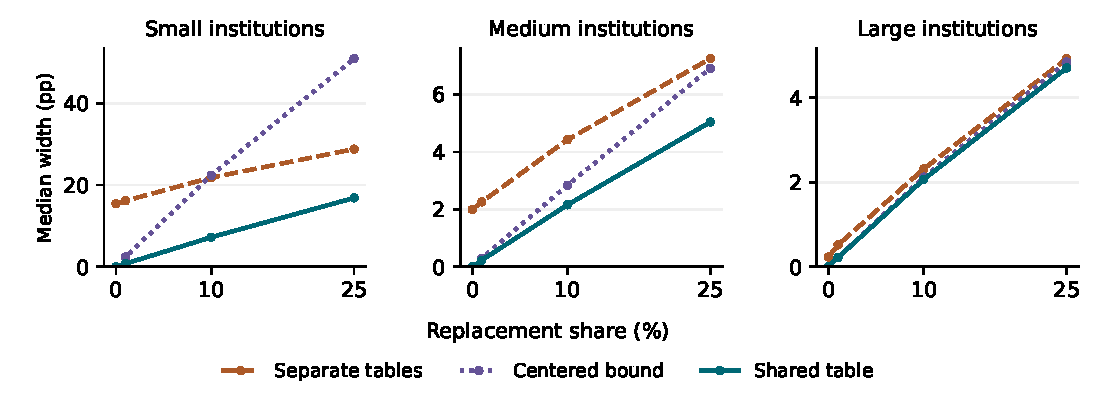
\includegraphics[width=.98\linewidth]{profiles.pdf}
\caption{Median widths with admissions rounded to tens. Each panel has its own vertical scale. Markers are evaluated radii; lines connect them for readability.}\label{fig:rho}
\end{figure}

\paragraph{When two recipients matter.}
At rounding to tens and $\rho=.10$, a single-site check misses an endpoint by more than 0.1 pp in only 1 of 60 portfolios (maximum 0.176 pp). At $\rho=.25$ the count rises to 20 of 60 (maximum 1.229 pp); at full replacement it is 50 of 60 (maximum 30.646 pp). Thus single-site checks can be numerically close at modest drift, yet they cannot certify their own accuracy. The median excess width of the certified linear-time enclosure over the exact range was 0.006, 0.546, 3.096 and 35.723 pp at replacement shares of 1, 10, 25 and 100\%, respectively. Its small-radius guarantee loses practical force at full replacement. In a single-process synthetic timing study on the same Windows host, the median of five warm runs at 256 sites was 0.34 ms for the scan and 777 ms for the pair solver. Both methods used the same interval table and radius of 0.10.

\paragraph{Noisy releases.}
The inverted count box covered all true cells in 579 of 600 runs. Both the sharp shared-table and separate-table envelopes covered both true extrema in all 600. Clipped noisy counts treated as exact enclosed the full truth in 163 of 600 (27.2\%). The 100 replicates per fixed panel have worst-case Monte Carlo standard error 5 percentage points for a coverage fraction. These are conditional simulation frequencies across six fixed panels; the formal 95\% lower guarantee follows from noise inversion. A plug-in range is a point estimate of two endpoints and has no nominal simultaneous coverage.
\begin{table}[ht]
\centering
\caption{Laplace simulation at $\rho=.10$. Coverage requires enclosing both true extrema. Widths are medians in percentage points. Each row pools two fixed panels.}
\begin{tabular}{lrrrrr}
\toprule
Size & Runs & Box covers table & Plug-in covers & Shared width & Separate width\\
\midrule
Small & 200 & 192 & 65 & 7.74 & 30.49\\
Medium & 200 & 192 & 39 & 1.61 & 3.04\\
Large & 200 & 195 & 59 & 4.06 & 4.25\\
\bottomrule
\end{tabular}
\end{table}

\subsection{Paired decisions after publishing exact totals}
We kept the 60 panels and the ten-percent replacement fraction fixed. In the follow-up release, each institution publishes exact application and admission totals, keeps its available group application counts public, and rounds available group admissions to tens. The criterion remained an entire signed change interval inside $[-5,+5]$ pp, including its endpoints. We specified the follow-up before computing the constrained endpoints, after observing the original 13 small-panel certifications.

\begin{table}[ht]
\centering
\caption{Panels certified at the same 5 pp tolerance. The scan uses a guaranteed outer interval. The final two columns refer to the subset previously certified by the exact algorithm.}
\label{tab:totals}
\begin{tabular}{lrrrrrr}
\toprule
&\multicolumn{2}{c}{Original release}&\multicolumn{2}{c}{Public total}&\multicolumn{2}{c}{Among original exact}\\
Size & Exact & Scan & Exact & Scan & Exact & Scan\\
\midrule
Small ($n=20$)  &13&9 &14&12&13/13&12/13\\
Medium ($n=20$) &20&20&20&20&20/20&20/20\\
Large ($n=20$)  &20&20&20&20&20/20&20/20\\
All ($n=60$)    &53&49&54&52&53/53&52/53\\
\bottomrule
\end{tabular}
\end{table}

Retention follows from nesting: a true public total can only remove feasible tables. The empirical results are the additional certification and the two exact-only decisions in Table~\ref{tab:totals}. In small panel 5 of 2022 the original upper endpoint was $+5.229$ pp. The total reduces it to $+4.814$ pp, while the scan still permits $+5.826$ pp. In small panel 9 of 2023 the exact interval already passed under the original release; with totals its upper endpoint is $+4.552$ pp and the scan's is $+5.425$ pp. The lower endpoints of both methods pass in these two cases. Withholding the residual admission cells while retaining the institution total and combined residual application capacity gives the same certification decisions. At an exploratory 7.5 pp tolerance both methods certify 18 of 20 small panels.

For small panels the median sharp width moves from 7.23 to 6.17 pp; the median \emph{paired} reduction is 0.67 pp. A simpler quadratic-time comparator projects each site polygon onto its two coordinates and applies the original rectangle algorithm. It makes the same 60 certification decisions at 5 pp. The largest endpoint difference from the polygon solution is 0.00064 pp or less. The observed decision gains primarily reflect tighter feasible cell ranges and the difference between an exact search and the conservative scan. Full polygon optimization supplies sharpness, with little additional numerical effect here. The study uses a simulated disclosure policy on public data and 60 constructed panels with 211 institutions shared between the two years.

\subsection{A next-year diagnostic and a named system}
This exploratory replay fixes the 2022 sites and obtains the observed 2023 application shares $w'$. Their smallest compatible replacement radius is
$\rho_*=\max_{s:b_s>0}(1-w'_s/b_s)_+$, since $w'_s\ge(1-\rho)b_s$ for every $s$. At that radius we compute both the entire 2022 composition envelope and the particular prediction $G(w';r_{22})-G(b;r_{22})$ with 2022 group shares. The observed change uses the actual 2023 rates and group shares.

Of 30 baseline portfolios, 24 had valid follow-up records at every site. The median required replacement fraction was 25.5\%. Five of the 24 realized changes fell outside the exact-count envelope; four fell outside even after rounding the original admissions to tens. Median absolute deviation between the realized change and the frozen-site prediction at the actual weights was 0.83 pp. An exceedance rules out the stipulated composition-only explanation for these recorded tables. Membership within the envelope cannot establish that explanation, because a different site mix may attain the same gap.

At the nine UC campuses $\rho_*=7.22\%$. The observed pooled gap changed by $-0.121$ pp. Transporting the unchanged 2022 site laws to the actual 2023 shares gives $-0.232$ pp, while the sharp exact-count interval at that radius is $[-0.497,+0.329]$ pp. Rounding to tens produces $[-0.503,+0.331]$ pp. Coarsening makes little practical difference in this large-volume system. Neither this exercise nor the panel construction adjusts for applicant qualifications or attributes a change to campus policy.

\end{document}
